\chapter{Problema Centralizado de Despacho Ótimo}
\localtableofcontents 

Este capítulo é baseado nas notas de aula do curso, ministrado em 10/08/2023, e nas informações do Capítulo 8 de \textcite{cretì_fontini_2019}.

\section{Introdução ao Problema}
Neste capítulo, analisamos o problema de fornecer eletricidade para atender à carga a partir de uma variedade de usinas de energia de maneira ótima. Como é comum em economia, consideramos a eficiência de Pareto como critério de otimização. Não levamos em conta externalidades, bens públicos e questões distribucionais.

Assuma que o sistema possui uma carga (\textit{load}) fixa $\overline{Q}>0$. Assuma um monopolista que detenha um número $I$ de usinas de geração elétrica com diferentes estruturas de custo $c_i(q_i)$. Defina o Bem-Estar Social como $W \equiv u(Q)-\sum_ic_i(Q)$, onde $u(\cdot)$ é a utilidade da sociedade com respeito ao consumo de eletricidade. Assuma, de forma geral e pelo resto do curso, as propriedades usuais para função custo e utilidade i.e. $u'(\cdot)>0, u''(\cdot)\le0,c'(\cdot)>0,c''(\cdot)\ge0,u(0)=0$.

Mais ainda, note que como a carga do sistema é tomada exogenamente i.e. os agentes (consumidores) consomem agregadamente uma quantidade fixa de eletricidade, independente de qualquer outro fator, temos que $W=u(\overline{Q})-\sum_ic_i(Q)$. Mais ainda, nesse contexto o problema do monopolista que minimiza custos é idêntico ao de um planejador central que maximiza o bem-estar. Essa relação é chamada de "problema dual", entretanto, não confunda com o problema dual das condições de KKT (ver Capítulo~\ref{kkt}).
\section{O Problema do Monopolista}
Explicitamente, assuma $I=2$. O problema do monopolista pode ser parcialmente escrito como:
\begin{align*}
    \min_{q_1,q_2\in\mathbb{R}}&\quad c_1(q_1) + c_2(q_2)\\
    \text{s.a.}&\quad 0\le q_1\le q_1^{max}\\
    &\quad 0\le q_2\le q_2^{max}\\
    &\quad 0\le q_1\le q_1^{max}\\
    &\quad q_1+q_2=\overline{Q}
\end{align*}
Podemos, então, escrever o Lagrangiano do problema como:
\begin{align*}
    \mathcal{L}=c_1(q_1) + c_2(q_2) +\mu(q_1+q_2-\overline{Q}) +\lambda_1 (-q_1) +\lambda_2 (-q_2) + \lambda_3(q_1-q_1^{max})+ \lambda_4(q_2-q_2^{max})    
\end{align*}

Como já assumimos que $c_i(\cdot)\ge0$ i.e. as funções custo são (quasi-)convexas, temos que as condições KKT são suficientes para determinar o ótimo do programa não-linear descrito acima. Explicitamente, as condições KKT para este problema são:
\begin{align*}
    \begin{aligned}
        \frac{\partial\mathcal{L}}{\partial q_1} &= c_1'(q_1) + \mu - \lambda_1 + \lambda_3 = 0\\
        \frac{\partial\mathcal{L}}{\partial q_2} &= c_2'(q_2) + \mu - \lambda_2 + \lambda_4 =0 
        \end{aligned} &&
        \left. \begin{aligned}
           \text{ }\\
           \text{ }
        \end{aligned}  \right\rbrace && \qquad \text{\textbf{Estacionariedade}}\\
        \begin{aligned}
            \lambda_1 (-q_1)&=0 \\
            \lambda_2 (-q_2)&=0 \\
            \lambda_3(q_1-q_1^{max})&=0\\
            \lambda_4(q_2-q_2^{max})&=0
        \end{aligned} &&
         \left. \begin{aligned}
           \text{ } \\
           \text{ } \\
           \text{ } \\
           \text{ } 
        \end{aligned}  \right\rbrace && \qquad \text{\textbf{Frouxidão Complementar}}\\
        \begin{aligned}
            \lambda_1,\lambda_2,\lambda_3,\lambda_4\ge0
        \end{aligned} &&
        \left. \begin{aligned}
           \text{ }
        \end{aligned}  \right\rbrace && \qquad \text{\textbf{Factibilidade Dual}}\\
        \begin{aligned}
            0\le q_1&\le q_1^{max}\\
            0\le q_2&\le q_2^{max}\\
            0\le q_1&\le q_1^{max}\\
            q_1+q_2&=\overline{Q}
        \end{aligned} && 
        \left. \begin{aligned}
           \text{ }\\
           \text{ }\\
           \text{ }\\
           \text{ } 
        \end{aligned}  \right\rbrace && \qquad \text{\textbf{Factibilidade Primal}}\\
\end{align*}
Suponha, com \textit{pouca perda de generalidade}, que $c_1'(q_1)<c_2'(q_2)$ para todo $q_1,q_2\in\mathbb{R}$. Note, entretanto, que, da forma como escrito acima, o problema é indefinido, ou seja, precisa de mais restrições. 

\subsection{Caso $q_1^{max},q_2^{max}>\overline{Q}$}
Repare que assumirmos $q_1^{max},q_2^{max}>\overline{Q}$ implica $q_1^*<q_1^{max}$ e $q_2^*<q_2^{max}$ pois, caso contrário, teríamos uma violação da factibilidade primal ($q_1^*+q_2^*>\overline{Q}$). Logo, pela frouxidão complementar, temos que $\lambda_3=\lambda_4=0$. Destarte, podemos reescrever as condições de estacionariedade da seguinte forma:
\begin{align*}
    \begin{cases}
        c_1'(q_1) = -\mu+\lambda_1\\
        c_2'(q_2) = -\mu+\lambda_2
    \end{cases}
\end{align*}
Teremos então que, de $c_1(\cdot)<c_2(\cdot)$:
\begin{align*}
     -\mu+\lambda_1< -\mu+\lambda_2 \Longleftrightarrow \lambda_1<\lambda_2
\end{align*}
Temos, portanto, dois possíveis casos para que a condição acima seja verdade.
\begin{enumerate}
    \item[1)] Suponha que $\lambda_1>0$ t.q. $\lambda_1<\lambda_2$. Ora, então teríamos, por frouxidão complementar, que $q_1^*=q_2^*=0$. Esse resultado claramente não atende factibilidade primária, pois implica $\overline{Q}=0$, e, portanto, não pode ser solução do problema de otimização. 
    \item[2)] Suponha que $\lambda_1=0$, implicando $\lambda_2>0$. Teríamos então, por frouxidão complementar, que $q_1^*>0$ e $q_2^*=0$ t.q. $q_1^*+q_2^*=\overline{Q}$ (por factibilidade primal), implicando por sua vez $q_1^*=\overline{Q}$. Repare que esse resultado atende à todas as condições KKT sendo, portanto, solução do problema de otimização.
\end{enumerate}
Concluímos, então, que a usina mais eficiente (com o menor custo marginal) é aquela que atende toda a carga exógena $\overline{Q}$. Em específico, supondo forma funcional
\[c_i(q_i)=FC_i+c_i'q_i\]
Temos a representação gráfica do problema dada pela Figura~\ref{fig:dispatching_1}.
\begin{figure}
    \centering
    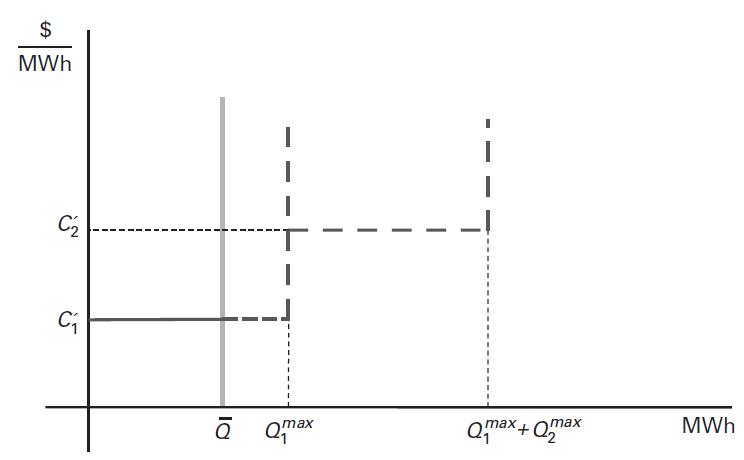
\includegraphics[scale=.4]{figure/dispatching_1.png}
    \caption{Despachamento Ótimo quando $q_1^{max},q_2^{max}>\overline{Q}$}
    \label{fig:dispatching_1}
\end{figure}

\subsection{Caso $q_1^{max},q_2^{max}<\overline{Q}$}
Repare que assumirmos $q_1^{max},q_2^{max}<\overline{Q}$ implica $q_1^*,q_2^*>0$, pois, caso contrário, teríamos uma violação da factibilidade primal ($q_1^*+q_2^*<\overline{Q}$). Logo, pela frouxidão complementar, temos que $\lambda_1=\lambda_2=0$. Destarte, podemos reescrever as condições de estacionariedade da seguinte forma:
\begin{align*}
    \begin{cases}
        c_1'(q_1) = -\mu-\lambda_3\\
        c_2'(q_2) = -\mu-\lambda_4
    \end{cases}
\end{align*}
Teremos então que, de $c_1(\cdot)<c_2(\cdot)$:
\begin{align*}
     -\mu-\lambda_3< -\mu-\lambda_4 \Longleftrightarrow \lambda_3>\lambda_4
\end{align*}
Temos, portanto, dois possíveis casos para que a condição acima seja verdade.
\begin{enumerate}
    \item[1)] Suponha que $\lambda_4>0$ t.q. $\lambda_3>\lambda_4$. Então temos, por frouxidão complementar, que $q_1^*<q_1^{max}$, $q_2^*<q_2^{max}$ e, por factibilidade primal, $q_1^*+q_2^*=\overline{Q}$ - implicando custo total $C^* = c_1(q_1^*)+c_2(q_2^*)$. 
    \item[2)] Suponha que $\lambda_4=0$. Teremos, por argumento similar ao do item anterior, $q_1^{**}=q_1^{max}$, $q_2^{**}<q_2^{max}$ e $q_1^{**}+q_2^{**}=\overline{Q}$, implicando $C^{**} = c_1(q_1^{max})+c_2(q_2^*)$.
\end{enumerate}
\begin{prop}
    Existem dois candidatos a mínimo global do problema do monopolista, nomeadamente, $C^*$ e $C^{**}$. O mínimo global é $C^{**}$, ou seja, $C^{**}<C^{*}$.
    \begin{proof}
        A forma mais rigorosa matematicamente de se demonstrar a proposição em questão seria demonstrar dominância estocástica de primeiro grau. De forma mais intuitiva (ainda que às custas de alguma generalidade), entretanto, podemos analisar que, pela expansão de Taylor de primeira ordem:
        \begin{align*}
            C^{**} &= c_1(q_1^{max}) + c_2(q_2^{**}) \\
            &\approx c_1(q_1^*) + c'(q_1^*)(q_1^{max}-q_1^*) + c_2(q_2^*) + c_2'(q_2^*)(q_2^{**}-q_2^*)\\
            &= C^* + c'(q_1^*)(q_1^{max}-q_1^*) + c_2'(q_2^*)(q_2^{**}-q_2^*)
        \end{align*}
        Note que, por factibilidade primal:
        \begin{align*}
            \underbrace{q_1^{max}+q_2^{**}}_{\overline{Q}} = \underbrace{q_1^*+q_2^*}_{\overline{Q}} \Longleftrightarrow q_1^{max}-q_1^* = -(q_2^{**}-q_2^*) \equiv \kappa >0
        \end{align*}
        Ora, aplicando na equação anterior temos que:
        \begin{align*}
            C^{**}-C^{*} \approx \kappa(c_1'(q_1^*)-c_2'(q_2^*))<0 \Rightarrow C^{**}<C^*
        \end{align*}
        Onde a negatividade seque de assumirmos desde o começo que $c_1'(\cdot)<c_2'(\cdot)$.
    \end{proof}
\end{prop}
Concluímos então que a usina mais eficiente (com menor custo marginal) opera em capacidade máxima, enquanto a menos eficiente opera de acordo a atender à carga exógena $\overline{Q}$. Supondo, novamente, forma funcional
\[c_i(q_i)=FC_i+c_i'q_i\]
Temos a representação gráfica do problema dada pela Figura~\ref{fig:dispatching_2}.
\begin{figure}
    \centering
    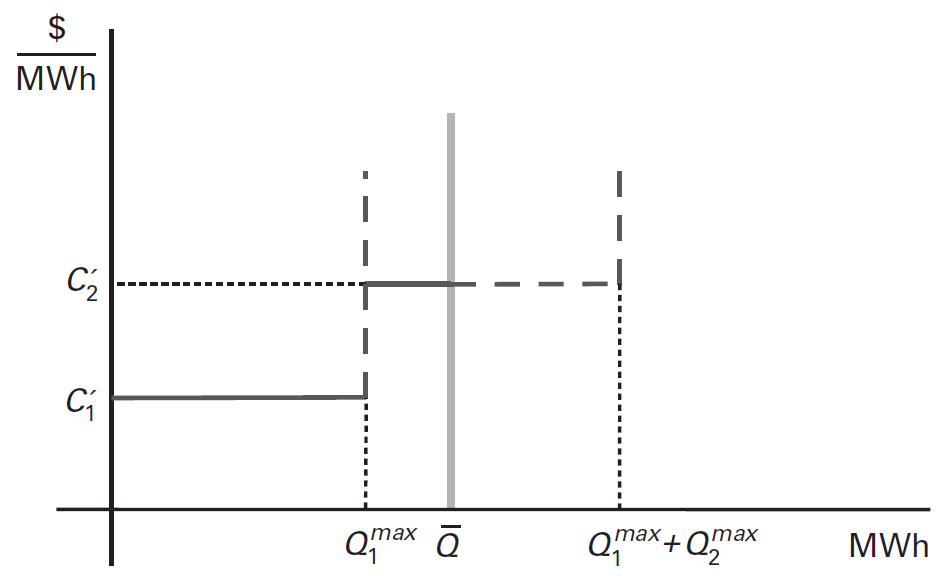
\includegraphics[scale=.3]{figure/dispatching_2.png}
    \caption{Despachamento Ótimo quando $q_1^{max},q_2^{max}<\overline{Q}$}
    \label{fig:dispatching_2}
\end{figure}

\section{Ordem de Mérito}
Os resultados discutidos acima são facilmente generalizáveis por indução para $i>2$ usinas. Isto é, dado que podemos ordenar as usinas em termos de eficiência (custo marginal), sem perda de generalidade, faça com que:
\[ c_1(\cdot)<c_2(\cdot)<\hdots<c_I(\cdot) \]

Teremos então que para uma dada carga exógena, as firmas mais eficientes serão ativadas, em ordem, até atenderem a carga $\overline{Q}$ ou alcançarem sua capacidade máxima.

\section{Custo Marginal do Sistema}
Repare que, no caso geral em que temos $I$ usinas, o Lagrangiano pode ser escrito como:
\[\mathcal{L}=\sum_{i=1}^Ic_i(q_i)+\mu\left(\sum_{i=1}^Iq_i-\overline{Q}\right)+\sum_{i=1}^I\lambda_i(-q_i) + \sum_{i=1}^{I}\lambda_{I+i}(q_i-q_i^{max})\]
Mais ainda, note que:
\[\frac{\partial\mathcal{L}}{\partial\overline{Q}}=-\mu\]
Ou seja, $\mu$ representa o custo que o monopolista (ou planejador) deve pagar \textit{na margem} para produzir a última (ou próxima) unidade marginal de eletricidade que atende à carga exógena $\overline{Q}$. Por este motivo, $\mu$ é chamado de Custo Marginal do Sistema.

Podemos repensar o resultado comentado da ordem de mérito com este conceito em mente. De forma geral, resolvendo o problema de otimização com o Lagrangiano acima, teremos 3 possibilidades para o valor de $c_i'(q_i)$:
\begin{align*}
     c_i'(q_i) =\begin{cases}
        -\mu+\lambda_i>-\mu&\text{caso $\lambda_{i}>0$ e $\lambda_{i+I}=0$} \\
        -\mu&\text{caso $\lambda_{i}=0$ e $\lambda_{i+I}=0$} \\
        -\mu-\lambda_{i+I}<-\mu&\text{caso $\lambda_{i}=0$ e $\lambda_{i+I}>0$}
    \end{cases}  
\end{align*}
De forma análoga aos exemplos com apenas duas usinas, poderemos concluir que a resposta ótima da usina $i$ é tal que:
\begin{align*}
    q_i^*=\begin{cases}
        q_i^{max} & \text{caso $c_i'(q_i)<-\mu$}\\
        \omega \in(0,q_i^{max}) & \text{caso $c_i'(q_i)=-\mu$}\\
        0 & \text{caso $c_i'(q_i)>-\mu$}
    \end{cases}
\end{align*}
Repare que essa intuição está em perfeito acordo com a ordem de mérito.

\section{Problema do Planejador Central}
Se flexibilizarmos a hipótese de que $\overline{Q}>0$ é exógeno e fixo, temos que a equivalência entre o Problema do Monopolista e o Problema do Planejador Central deixa de valer. Entretanto, as similaridades entre ambos problemas é notável em virtude da linearidade do problema. Assuma, sem perda de generalidade, que existam $N$ consumidores e que $U(q^1,\hdots,q^N)=\sum_{n=1}^Nu^n(q^n)$. Podemos escrever o Problema do Planejador Central como:
\begin{align*}
    \max_{\substack{q_1,\hdots,q_I\in\mathbb{R}\\q^1\hdots q^N\in\mathbb{R}}}&\quad \sum_{n=1}^Nu^n(q^n) - \sum_{i=1}^Ic_i(q_i)\\
    \text{s.a}&\quad \sum_nq^n=\sum_iq_i\\
    &\quad 0\le q_i \le q_i^{max},\quad \forall i=1,\hdots,I\\
    &\quad 0\le q^n \le q^{n^{max}},\quad \forall n=1,\hdots,N
\end{align*}
Implicando o seguinte Lagrangiano: 
\begin{align*}
    \mathcal{L}=\sum_ic_i(q_i)-\sum_nu^n(q^n)+\mu\left(\sum_iq_i-\sum_nq^n\right)&+\sum_i\lambda_i(-q_i) + \sum_i\lambda_{I+i}(q_i-q_i^{max})\\
    &+\sum_{n}\gamma_n(-q^n) + \sum_n\gamma_{N+n}(q^n-q^{n^{max}})
\end{align*}
Segue, de forma exatamente análoga à seção anterior, que:
\begin{align*}
    q^{n^*}=\begin{cases}
        q^{n^{max}} & \text{caso $u^{n'}(q^n)>\mu$}\\
        \eta \in(0,q^{n^{max}}) & \text{caso $u^{n'}(q^n)=\mu$}\\
        0 & \text{caso $u^{n'}(q^n)<\mu$}
    \end{cases}
\end{align*}
Ou seja, a carga do sistema segue funções de reação similares às de oferta de eletricidade e, destarte, deve atender à ordem de mérito de forma que os agentes com maior utilidade marginal são supridos primeiro, em ordem.